%% abtex2-modelo-include-comandos.tex, v-1.9.5 laurocesar
%% Copyright 2012-2015 by abnTeX2 group at http://www.abntex.net.br/ 
%%
%% This work may be distributed and/or modified under the
%% conditions of the LaTeX Project Public License, either version 1.3
%% of this license or (at your option) any later version.
%% The latest version of this license is in
%%   http://www.latex-project.org/lppl.txt
%% and version 1.3 or later is part of all distributions of LaTeX
%% version 2005/12/01 or later.
%%
%% This work has the LPPL maintenance status `maintained'.
%% 
%% The Current Maintainer of this work is the abnTeX2 team, led
%% by Lauro César Araujo. Further information are available on 
%% http://www.abntex.net.br/
%%
%% This work consists of the files abntex2-modelo-include-comandos.tex
%% and abntex2-modelo-img-marca.pdf
%%

% ---
% Este capítulo, utilizado por diferentes exemplos do abnTeX2, ilustra o uso de
% comandos do abnTeX2 e de LaTeX.
% ---

%\chapter{Resultados de comandos}\label{cap_exemplos}
\chapter{Introduction}\label{aboutTheProblem}
\noindent
State-space search algorithms have been used to solve important real-world problems, such as problems arising in Robotics, domain-independent planning, chemistry, biology, and engineering. For example, in Figure \ref{fig:example_fix} the agent, in the top-right requires to do a plan for the shortest path from the initial location to the location marked with the letter \texttt{g} (bottom-left corner); the shaded area represents an obstacle the agent cannot pass. The agent has two options to go to the goal: It can go to the location \texttt{b} or location \texttt{c}. The agent are going to find the shortest path going through c, because there is not obstacle to the goal. 

\begin{figure}[h]
\centering
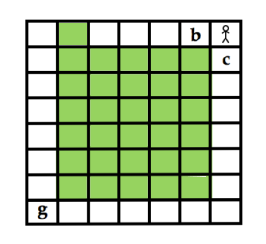
\includegraphics[width=8cm]{images/editarExampleLevi-Green}
\caption{The agent in the top-right corner requires to do a plan path to the location marked with a letter \texttt{g}; the shaded area represents an obstacle the agent cannot pass.} \label{fig:example_fix}
\end{figure}

In this dissertation we study methods for selecting a subset of heuristic functions while minimizing the search tree size and the running time of the A$\sp{*}$ \cite{hart1968formal} search algorithm while solving state-space search problems.

We are interested in selecting heuristics from a large set of possibilities because Holte et al., (\citeyear{holte2006maximizing}) showed that search can be faster if several smaller pattern databases are used instead of one large pattern database. %In fact, we believe that different heuristics can give us valuable information about the solution of the problem. For example, 
Intuitively, one heuristic can be helpful in a region of the search tree where another heuristic isn't. Then, instead of using one heuristic to find the solution, it would be best to use the most promising subset of heuristics from a possibly large set.

\section{Background work}
\noindent
State-space search algorithms are used to solve certain class of Artificial Intelligence (\texttt{AI}) problems by finding a sequence of actions from the start state to a goal state in the search space. Two well know search algorithms for solving state-space search problems are Depth-First Search (\texttt{DFS}) and Breadth-First Search (\texttt{BFS}). \texttt{DFS} looks for the solution by exploring the subtree rooted node $n$ before exploring the subtrees rooted at $n$'s siblings while looking for a path from start to goal. 

Figure \ref{fig:dfs_solution} shows the ordering in which \texttt{DFS} expands nodes while solving the 8-tile puzzle (explained in detail in Chapter~\ref{ch:background}), a state-space problem. We can see that \texttt{DFS} expands 31 states before finding a goal state (represented by the bottom right state). \texttt{BFS} looks for the solution by exploring all nodes in a given level before exploring nodes in the next level. In Figure \ref{fig:bfs_solution} we can see \texttt{BFS} expands 46 states to find the goal. In both Figure \ref{fig:dfs_solution} and Figure \ref{fig:bfs_solution} the numbers above of each state represent the order in which the states are visited. \texttt{DFS} and \texttt{BFS} are brute-force search algorithms, as they visit all states encountered during its search before finding a solution. %usually visit a large number of states before finding a solution. 
We call brute-force-search tree (\texttt{BFST}) the tree expanded by \texttt{DFS} and \texttt{BFS}.

\iftrue
\begin{landscape}

\begin{figure}[htb]
%\centering
\begin{forest}
%for tree={
%  parent anchor=south,
%  child anchor=north,
%}
[\usebox\myboxone
  [\usebox\myboxtwo
    [\usebox\myboxthree
		[\usebox\myboxfour
			[\usebox\myboxfive
				[\usebox\myboxsix]
				[\usebox\myboxseven]			
			]
		]
		[\usebox\myboxeight
			[\usebox\myboxnine
				[\usebox\myboxten]
				[\usebox\myboxeleven]			
			]
			[\usebox\myboxtwelve
				[\usebox\myboxthirteen]
				[\usebox\myboxfourteen]			
			]
			[\usebox\myboxfifteen
				[\usebox\myboxsixteen]
				[\usebox\myboxseventeen]
			]		
		]  
    ]
  ]
  [\usebox\myboxeighteen
	[\usebox\myboxnineteen
		[\usebox\myboxtwenty
			[\usebox\myboxtwentyone
				[\usebox\myboxtwentytwo]
				[\usebox\myboxtwentythree]			
			]		
		]
		[\usebox\myboxtwentyfour
			[\usebox\myboxtwentyfive
				[\usebox\myboxtwentysix]
				[\usebox\myboxtwentyseven]			
			]		
		]	
	]
	[\usebox\myboxtwentyeight
		[\usebox\myboxtwentynine
			[\usebox\myboxthirty
				[\usebox\myboxthirtyone]
			]		
		]	
	]  
  ]
]
\end{forest}
\caption{8 tile puzzle using DFS. \cite{bernard2011}} \label{fig:dfs_solution}
\end{figure}
\end{landscape}
\fi

\iftrue
\begin{landscape}
\begin{figure}[htb]
%\centering

%\resizebox{.5\linewidth}{!}{%
%\resizebox{\linewidth}{!}{%
\resizebox{\dimexpr\linewidth-1cm}{!}{%
\begin{forest}
%for tree={
%  parent anchor=south,
%  child anchor=north,
%}
[\usebox\myboxbfsone
  [\usebox\myboxbfstwo
	[\usebox\myboxbfsfive
		[\usebox\myboxbfsten
			[\usebox\myboxbfstwenty
				[\usebox\myboxbfsthirtyfour]
				[\usebox\myboxbfsthirtyfive]			
			]		
		]
		[\usebox\myboxbfseleven
			[\usebox\myboxbfstwentyone
				[\usebox\myboxbfsthirtysix]
				[\usebox\myboxbfsthirtyseven]			
			]
			[\usebox\myboxbfstwentytwo
				[\usebox\myboxbfsthirtyeight]
				[\usebox\myboxbfsthirtynine]			
			]
			[\usebox\myboxbfstwentythree
				[\usebox\myboxbfsforty]
				[\usebox\myboxbfsfortyone]			
			]		
		]	
	]  
  ]
  [\usebox\myboxbfsthree
	[\usebox\myboxbfssix
		[\usebox\myboxbfstwelve
			[\usebox\myboxbfstwentyfour
				[\usebox\myboxbfsfortytwo]
				[\usebox\myboxbfsfortythree]			
			]		
		]
		[\usebox\myboxbfsthirteen
			[\usebox\myboxbfstwentyfive
				[\usebox\myboxbfsfortyfour]
				[\usebox\myboxbfsfortyfive]			
			]		
		]	
	]
	[\usebox\myboxbfsseven
		[\usebox\myboxbfsfourteen
			[\usebox\myboxbfstwentysix
				[\usebox\myboxbfsfortysix]			
			]		
		]
		[\usebox\myboxbfsfifteen
			[\usebox\myboxbfstwentyseven]		
		]	
	]
	[\usebox\myboxbfseight
		[\usebox\myboxbfssixteen
			[\usebox\myboxbfstwentyeight]		
		]
		[\usebox\myboxbfsseventeen
			[\usebox\myboxbfstwentynine]		
		]	
	]  
  ]
  [\usebox\myboxbfsfour
	[\usebox\myboxbfsnine
		[\usebox\myboxbfseighteen
			[\usebox\myboxbfsthirty]
			[\usebox\myboxbfsthirtyone]
			[\usebox\myboxbfsthirtytwo]
		]
		[\usebox\myboxbfsnineteen
			[\usebox\myboxbfsthirtythree]		
		]
	]  
  ]
]
\end{forest}
}
\caption{8 tile puzzle using BFS. \cite{bernard2011}} \label{fig:bfs_solution}
\end{figure}
\end{landscape}
\fi

There are other types of algorithms called heuristic search algorithms, and the most representative algorithm of this type is A$\sp{*}$ \cite{hart1968formal}. % which also solves problems optimally. 
Heuristic search algorithms use a heuristic function for estimating the distance of a node in the search tree to a goal state. Heuristic search algorithms tend to generate smaller search trees than the \texttt{BFST} because the heuristic guides the search to more promising parts of the state space. Also, by reducing the search tree size, the guidance of the heuristic function might also reduce the overall running time of the algorithm.

There are different approaches (\citeauthor{haslum2007domain} \citeyear{haslum2007domain}; \citeauthor{edelkamp2007automated} \citeyear{edelkamp2007automated}; \citeauthor{nissim2011computing} \citeyear{nissim2011computing}) for creating heuristics. %The way to create heuristics could be with domain knowledge or without domain knowledge. %The systems that generate a heuristic are called heuristic generators by Barley et al., (\citeyear{BarleySantiagoOver}). 
One approach that has shown successful results in heuristic generation is Pattern Database (\texttt{PDB}) \cite{culberson1998pattern}. The way how \texttt{PDBs} work is as follows: The search space of the problem is abstracted into a smaller state space that can be enumerated with exhaustive search. The distance of all abstracted states to the abstracted goal state are stored in a lookup table, which can be used as a heuristic function for the original state space.

%Another approach is Genetic Algorithm (\texttt{GA}), proposed by Edelkamp, \citeyear{edelkamp2007automated}. Given a set of initial heuristics, in each iteration \texttt{GA} selects the heuristics that optimize certain fitness function.


\iffalse
\begin{figure}[htb]
\centering 
\begin{tikzpicture}

% -- center, xdim, ydim
\draw[very thick,cyan] \boundellipse{4,0}{6}{2};
\draw[very thick,cyan] \boundellipse{4,4}{3}{1};
	
  % First, define nodes
% -- points F
  
  \draw (-2,3) node[circle, inner sep=0.8pt, fill=cyan, label={{}}] (E) {E};  
  \draw (6,1) node[circle, inner sep=0.8pt, fill=cyan, label={{}}] (F) {F}; 

  \draw[very thick,cyan, ->>]  (E) .. controls +(5,-3) and +(-4,1).. (F);
  \path  ($(E)+(0,0.2)$) .. controls +(5,-3) and +(-4,1)..  ($(F)+(0,0.2)$) 
     {\foreach \i in {1,...,40} {  coordinate[pos=0.15+0.75*\i/40] (p\i) } };

  \draw (-1,2) node[circle, inner sep=0.8pt, fill=cyan, label={{}}] (A) {A};
  \draw[very thick,cyan, ->>]  (A) .. controls +(5,-3) and +(-4,1).. (F);
  \path  ($(A)+(0,0.2)$) .. controls +(5,-3) and +(-4,1)..  ($(F)+(0,0.2)$) 
     {\foreach \i in {1,...,40} {  coordinate[pos=0.15+0.75*\i/40] (p\i) } };
	
  \draw (-3,0) node[circle, inner sep=0.8pt, fill=cyan, label={{}}] (B) {B};
  \draw[very thick,cyan, ->>]  (B) .. controls +(5,-3) and +(-4,1).. (F);
  \path  ($(B)+(0,0.2)$) .. controls +(5,-3) and +(-4,1)..  ($(F)+(0,0.2)$) 
     {\foreach \i in {1,...,40} {  coordinate[pos=0.15+0.75*\i/40] (p\i) } };
	
% -- points in G

  \draw (-2,1) node[circle, inner sep=0.8pt, fill=cyan, label={{}}] (C) {C};
  \draw (6.5,0) node[circle, inner sep=0.8pt, fill=cyan, label={{}}] (G) {G};
  \draw[very thick,cyan, ->>]  (C) .. controls +(5,-3) and +(-4,1).. (G);
  \path  ($(C)+(0,0.2)$) .. controls +(5,-3) and +(-4,1)..  ($(G)+(0,0.2)$) 
     {\foreach \i in {1,...,40} {  coordinate[pos=0.15+0.75*\i/40] (p\i) } };	

\draw (-1,0) node[circle, inner sep=0.8pt, fill=cyan, label={{}}] (D) {D};	
\draw[very thick,cyan, ->>]  (D) .. controls +(5,-3) and +(-4,1).. (G);
  \path  ($(C)+(0,0.2)$) .. controls +(5,-3) and +(-4,1)..  ($(G)+(0,0.2)$) 
     {\foreach \i in {1,...,40} {  coordinate[pos=0.15+0.75*\i/40] (p\i) } };	

\draw (-3,-1) node[circle, inner sep=0.8pt, fill=cyan, label={{}}] (H) {H};	
\draw[very thick,cyan, ->>]  (H) .. controls +(5,-3) and +(-4,1).. (G);
  \path  ($(C)+(0,0.2)$) .. controls +(5,-3) and +(-4,1)..  ($(G)+(0,0.2)$) 
     {\foreach \i in {1,...,40} {  coordinate[pos=0.15+0.75*\i/40] (p\i) } };
	
% -- X
\draw (-2,-2) node[circle, inner sep=0.8pt, fill=cyan, label={{}}] (J) {J};
  \draw (6,-1) node[circle, inner sep=0.8pt, fill=cyan, label={{}}] (X) {X};
  \draw[very thick,cyan, ->>]  (J) .. controls +(5,-3) and +(-4,1).. (X);
  \path  ($(C)+(0,0.2)$) .. controls +(5,-3) and +(-4,1)..  ($(G)+(0,0.2)$) 
     {\foreach \i in {1,...,40} {  coordinate[pos=0.15+0.75*\i/40] (p\i) } };

\draw (-2,-3) node[circle, inner sep=0.8pt, fill=cyan, label={{}}] (K) {K};
\draw[very thick,cyan, ->>]  (K) .. controls +(5,-3) and +(-4,1).. (X);
  \path  ($(C)+(0,0.2)$) .. controls +(5,-3) and +(-4,1)..  ($(G)+(0,0.2)$) 
     {\foreach \i in {1,...,40} {  coordinate[pos=0.15+0.75*\i/40] (p\i) } };

%$\node [xshift=1cm,yshift=2cm] (A) at (-3,3) {Search Space};$
%$\node [xshift=1cm,yshift=2cm] (A) at (5,1) {Type System};$
	
\end{tikzpicture}
\caption{\texttt{PDB} approach} \label{fig:ss_ts}
\end{figure}
\fi

%Holte et al., (\citeyear{holte2006maximizing}) showed that search can be faster if several smaller \texttt{PDBs} are used instead of one large pattern database. In addition Domshlak et al., (\citeyear{domshlak2010max}) and Tolpin et al.,  (\citeyear{tolpin2013towards}) showed that evaluating the heuristic lazily, only when they are essential to a decision to be made in the search process, is worthy in comparison to take the maximum of the set of heuristics.
% ---
\section{Objectives}
%\subsection{Aim}
%\noindent
The objective of this dissertation is to develop algorithms for selecting a heuristic subset from a large set of heuristics with the goal of solving domain-independent planning problems. Specifically our objectives are the following. 

%\subsection{Objectives}
%\noindent

\begin{itemize}
  \item Develop a method to find a subset of heuristics from a large pool of heuristics $\zeta$ that minimizes the number of nodes expanded by A$\sp{*}$ in the process of search.
  
  \item Develop a method to find a subset of heuristics from a large pool of heuristics $\zeta$ that minimizes the A$\sp{*}$ running time.

\end{itemize}
% ---
\section{Scope, Limitations, and Delimitations}
\noindent
We implemented our method in Fast Downward \cite{helmert2006fast} and we tested our methods on the 2011 International Planning Competition (\texttt{IPC}) problem instances.

\section{Justification}
\noindent
Good results have been obtained in domain-independent planning by using heuristic search approach \cite{bonet2001planning}. The heuristic function used to guide the A$\sp{*}$ search are known to greatly affect the algorithm's running time. That is why it is important to have methods for selecting a good subset of heuristics to guide the A* search.

%We use heuristic generators in order to create a large set of heuristics and obtain heuristics to solve problems.

\section{Hypothesis}
\noindent
We test the following hypothesis:
\begin{itemize}
\item A greedy algorithm is effective for selecting a good subset of heuristics to guide the A* search.
\end{itemize}

\section{Contributions}
\noindent
The main contributions of this dissertation are:
\begin{itemize}
\item A meta-reasoning approach for selecting heuristic functions while minimizing the number of nodes generated by A$\sp{*}$.

\item A meta-reasoning approach for selecting heuristic functions while minimizing the running time of the A$\sp{*}$ search. 

\item Detailed experiments on domain-independent planning showing the strengths and weaknesses of the proposed approaches. Our experiments also show that one of our proposed approaches is able to outperform all other systems tested. 

\end{itemize}

\section{Organization}
\noindent
This dissertation is organized as follows: 
\begin{enumerate}
\item In Chapter I, the background of the dissertation is provided, which also includes the objectives and the scope definition.
\item In Chapter II we review the state-of-the-art in selection of heuristic functions.
\item In Chapter III we introduce Greedy Heuristic Selection (\texttt{GHS}). 
\item In Chapter IV compare \texttt{GHS} with other planner systems.
\item We conclude in Chapter V.
\end{enumerate}

%\clearpage